\documentclass[12pt, a4paper, twoside, titlepage]{article}
\usepackage[utf8]{inputenc}
\usepackage[english]{babel}
\usepackage{amsmath}
\usepackage{amsfonts}
\usepackage{amssymb}
\usepackage{graphicx}
\usepackage[dvipsnames]{xcolor}
\usepackage{tikz}
\usetikzlibrary{arrows,automata,shapes}
\tikzstyle{decision} = [diamond, draw, fill=blue!20, text width=4.5em, text badly centered, node distance=2.5cm, inner sep=0pt]
\tikzstyle{block} = [rectangle, draw, fill=blue!20, text width=5em, text centered, rounded corners, minimum height=4em]
\tikzstyle{line} = [draw, very thick, color=black!50, -latex']
\tikzstyle{cloud} = [draw, ellipse,fill=red!20, node distance=2.5cm,minimum height=2em]

\title{Libre Silicon process specification}
\date{\today} 
\author{David Lanzendörfer}

\begin{document}
\maketitle

\begin{abstract}
	Copyright © 2017 LANCEVILLE TECHNOLOGY GROUP CO., LIMITED. All rights reserved. \\

	This process is licensed under the Libre Silicon public license; you can redistribute it and/or modify it under the terms of the Libre Silicon public license
	as published by the Libre Silicon alliance, either version 2 of the License, or (at your option) any later version.

	This design is distributed in the hope that it will be useful, but WITHOUT ANY WARRANTY; without even the implied warranty of MERCHANTABILITY or FITNESS FOR A PARTICULAR PURPOSE.
	See the Libre Silicon Public License for more details. \\

	This is the specification of the free silicon manufacturing standard for manufacturing the ls018\footnotemark standard logic cells and related free technology nodes from the LibreSilicon project.
	\footnotetext[1]{https://github.com/leviathanch/ls018}
\end{abstract}

\section{Overall process}
Below the general flow chart of the overall process flow can be seen. These process steps will be discussed within the following sections.
\begin{center}
	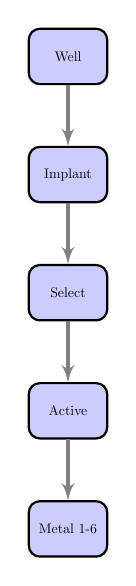
\begin{tikzpicture}[node distance = 3cm, auto, thick,scale=0.5, every node/.style={transform shape}]
		% Place nodes
		\node [block] (well) {Well};
		\node [block, below of=well] (implant) {Implant};
		\node [block, below of=implant] (select) {Select};
		\node [block, below of=select] (active) {Active};
		\node [block, below of=active] (metal) {Metal 1-6};
		% Draw edges
		\path [line] (well) -- (implant);
		\path [line] (implant) -- (select);
		\path [line] (select) -- (active);
		\path [line] (active) -- (metal);
	\end{tikzpicture}
\end{center}

The four starting overall process steps are part of an overall active part of the technology, while the final metal (respectively contact) layers will be used for making a contact between the logic gates and macro cells and making them available to the exterior world.
For this process p-substrate is the required basic substrate, but forks and modifications will be very well possible based on a Graphene substrate or alike, still under the LSPL.

\section{Well}
\subsection{Oxide layer}
In order to selectively inject charge carrying atoms into the crystalline structure a protective oxide layer needs to be grown on top of a p-type substrate.
\begin{center}
	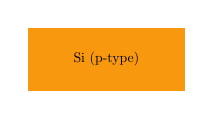
\begin{tikzpicture}[node distance = 3cm, auto, thick,scale=0.5, every node/.style={transform shape}]
		% substrate
		\fill[YellowOrange] (0,0) rectangle (4,1.6);
		\node at (2,0.8) {Si (p-type)};
	\end{tikzpicture}
	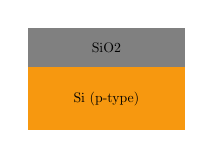
\begin{tikzpicture}[node distance = 3cm, auto, thick,scale=0.5, every node/.style={transform shape}]
		% substrate
		\fill[YellowOrange] (0,0) rectangle (4,1.6);
		\node at (2,0.8) {Si (p-type)};
		% oxide
		\fill[gray] (0,1.6) rectangle (4,2.6);
		\node at (2,2.1) {SiO2};
	\end{tikzpicture}
	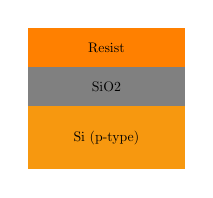
\begin{tikzpicture}[node distance = 3cm, auto, thick,scale=0.5, every node/.style={transform shape}]
		% substrate
		\fill[YellowOrange] (0,0) rectangle (4,1.6);
		\node at (2,0.8) {Si (p-type)};
		% oxide
		\fill[gray] (0,1.6) rectangle (4,2.6);
		\node at (2,2.1) {SiO2};
		% resist
		\fill[orange] (0,2.6) rectangle (4,3.6);
		\node at (2,3.1) {Resist};
	\end{tikzpicture}
\end{center}
\subsection{Pattering and etching}
\begin{center}
	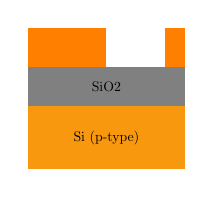
\begin{tikzpicture}[node distance = 3cm, auto, thick,scale=0.5, every node/.style={transform shape}]
		% substrate
		\fill[YellowOrange] (0,0) rectangle (4,1.6);
		\node at (2,0.8) {Si (p-type)};
		% oxide
		\fill[gray] (0,1.6) rectangle (4,2.6);
		\node at (2,2.1) {SiO2};
		% resist 1
		\fill[orange] (0,2.6) rectangle (2,3.6);
		% resist 2
		\fill[orange] (3.5,2.6) rectangle (4,3.6);
	\end{tikzpicture}
\end{center}
\subsection{Infusion}

\section{Implant}
\section{Select}
\section{Active}
\section{Metal}


\end{document}